\documentclass[11pt]{article}
\usepackage[margin=1in]{geometry}
\usepackage{graphicx,booktabs,xcolor,authblk,lineno,amsmath,amssymb}
\usepackage[numbers,sort&compress]{natbib}
\usepackage[hidelinks]{hyperref}
\usepackage{url}
\urlstyle{tt}
\newcommand{\code}[1]{\nolinkurl{#1}}  % monospace code that can break across lines
\graphicspath{{figures/}}
\emergencystretch=2em  % let TeX loosen lines rather than overflow the margin
\newcommand{\todo}[1]{{\color{red}[#1]}}  % marks placeholders in red
% float pages: start each figure at the top of its page (default centers it vertically)
\makeatletter
\setlength{\@fptop}{0pt}
\setlength{\@fpsep}{8pt plus 1fil}
\setlength{\@fpbot}{0pt plus 1fil}
\makeatother

% author block: larger author names, compact footnote-size affiliations, tighter spacing
\renewcommand\Authfont{\normalsize}
\renewcommand\Affilfont{\footnotesize}
\renewcommand\Authsep{, }
\renewcommand\Authand{ and }
\renewcommand\Authands{, and }
\setlength{\affilsep}{0.6em}
\title{Pycea: a scverse toolkit for single-cell lineage tracing analysis}
\author[1,2]{William~N. Colgan}
\author[3]{Eric Weine}
\author[2,4]{Matthew~G. Jones}
\author[1,2,4,5]{Jonathan~S. Weissman}
\author[6,*]{Nir~Yosef}
\affil[1]{Whitehead Institute for Biomedical Research, Cambridge, MA, USA}
\affil[2]{Department of Biology, MIT, Cambridge, MA, USA}
\affil[3]{Department of Electrical Engineering and Computer Sciences, MIT, Cambridge, MA, USA}
\affil[4]{David H. Koch Center for Integrative Cancer Research, MIT, Cambridge, MA, USA}
\affil[5]{Howard Hughes Medical Institute, Chevy Chase, MD 20815, USA}
\affil[6]{Department of Systems Immunology, Weizmann Institute of Science, 7610001 Rehovot, Israel}
\affil[*]{Corresponding author: Nir Yosef, nir.yosef@weizmann.ac.il}
\date{\small Email addresses: WNC, wcolgan@wi.mit.edu; EW, eric\_weine@dfci.harvard.edu; MGJ, mgjones@mit.edu; JSW, weissman@wi.mit.edu; NY, nir.yosef@weizmann.ac.il}

\begin{document}
\maketitle
\linenumbers

\begin{abstract}
% Abstract
Lineage tracing enables reconstruction of cellular histories in development, regeneration, and disease, but integrating lineage data into single-cell analysis workflows remains challenging. We introduce Pycea, a Python toolkit for lineage analysis and visualization, and TreeData, an extension of AnnData that stores lineage trees alongside cellular measurements. TreeData is compatible with Scanpy and other scverse tools, enabling integrated analysis without converting between formats. Pycea provides scalable methods for tree visualization, clade identification, distance comparisons, ancestral state inference, and lineage statistics. This software is open source and available at \url{https://github.com/YosefLab/pycea}.
\end{abstract}

\noindent\textbf{Keywords:} lineage tracing, live-cell tracking, single-cell, scRNA-seq, scverse, AnnData

\section*{Background}% introduction
Technological advances have dramatically increased the acquisition of single-cell lineage tracing data, with recently published studies including more than one million cells \citep{yu2026typewriter,colgan2026}. These datasets combine measurements of individual cells with lineage trees describing their division histories and can be generated through live-cell tracking or molecular recording. In live-cell tracking, cell movements are directly observed using time-lapse microscopy, allowing lineage trees to be reconstructed from observed cell divisions \citep{sulston1983lineage,keller2008zebrafish,mcdole2018intoto,ulman2017tracking,ershov2022trackmate}. In molecular recording, cells are engineered to accumulate heritable genomic marks that can subsequently be used to reconstruct their lineage relationships. These marks can be introduced using CRISPR--Cas9 \citep{mckenna2016gestalt,chan2019molecular,bowling2020carlin,frieda2017memoir,chow2021intmemoir}, prime editing \citep{choi2022typewriter,koblan2025}, or base editing \citep{hwang2019l1,winter2026baseline}. Both approaches can pair lineage information with additional cellular measurements, including gene expression \citep{raj2018scgestalt,spanjaard2018linnaeus,bowling2020carlin,colgan2026}, spatial coordinates \citep{koblan2025}, and cell morphology, enabling the study of cell states and behaviors across development, regeneration, and disease.

The scverse ecosystem has established a common framework for single-cell RNA-seq (scRNA-seq) analysis in Python \citep{virshup2023scverse}, centered on AnnData, a standardized data structure for storing single-cell measurements and associated metadata \citep{virshup2024anndata}. Extensions such as MuData and SpatialData add support for multimodal and spatial datasets \citep{bredikhin2022muon,marconato2024spatialdata}. These interoperable data structures support a growing ecosystem of tools, including Scanpy \citep{wolf2018scanpy} and Squidpy \citep{palla2022squidpy}, allowing users to process, visualize, and analyze single-cell data without repeatedly converting between formats. However, the scverse ecosystem has lacked a standardized data structure for lineage trees, making it difficult to integrate lineage analysis into existing single-cell workflows.

Existing tools such as LinTIMaT, DCLEAR, Startle, TiDeTree, and LAML primarily focus on lineage tree reconstruction \citep{zafar2020lintimat,gong2022dclear,sashittal2023startle,seidel2022tidetree,chu2025laml,chu2026lamlpro}. Our Cassiopeia package \citep{jones2020cassiopeia} additionally provides some plotting and analysis functionality, but integrating gene expression data is cumbersome because the \code{CassiopeiaTree} object does not natively store this modality or integrate with the scverse ecosystem. Similarly, users performing lineage analysis with phylogenetic tools such as ETE \citep{huertacepas2016ete} need to manually transfer cell annotations, such as Leiden clusters, from AnnData into the ETE \code{Tree} object. Our goal is to eliminate this data juggling and enable seamless analysis of lineage trees alongside gene expression and other features.

Here, we introduce Pycea, a scverse-compatible toolkit for lineage analysis and visualization built around TreeData, an extension of AnnData that supports the storage of lineage trees alongside other single-cell measurements. TreeData serves as a drop-in replacement for AnnData, retaining compatibility with Scanpy and other scverse tools while enabling integrated lineage analysis. Pycea provides a suite of intuitive and scalable methods for visualizing lineage trees, identifying clades, comparing lineage distances, inferring ancestral states, and more. We demonstrate these capabilities using lineage tracing datasets from mouse development and a metastatic tumor model \citep{colgan2026,koblan2025}. Additional examples and documentation are available in the Pycea documentation \citep{pycea_docs}.

\section*{Results}% results
\subsection*{TreeData stores lineage trees alongside other single-cell measurements}

To integrate lineage trees into standard single-cell workflows, we developed TreeData, an extension of AnnData that adds support for storing trees (Figure~2A). TreeData adds two fields, \code{obst} and \code{vart}, which store trees as \code{networkx} directed graphs \citep{hagberg2008networkx} aligned with observations (cells) and variables (genes), respectively. Node and edge attributes, such as node time, are stored as key-value pairs on the tree. The AnnData interface (\code{X}, \code{obs}, \code{var}, \code{obsm}, \code{varm}, \code{layers}, \code{uns}, etc.) remains unchanged, and because TreeData is a subclass of AnnData, it can be passed directly to Scanpy, Squidpy, and other scverse tools. TreeData objects can be saved to disk as \code{.h5td} or \code{.zarr} files, with I/O times comparable to AnnData, particularly for scRNA-seq data where expression matrices dominate I/O (Figure~S1A).

TreeData supports three \code{alignment} options (Figure~2B): (1) \code{"leaves"} indicates that observations correspond to the leaves of the tree, as is typically the case for molecular recording; (2) \code{"nodes"} indicates that both leaves and internal nodes correspond to observations, as is typically the case for live-cell tracking; and (3) \code{"subset"} indicates that only a subset of nodes correspond to observations (see \code{pycea.datasets.packer19} for an example in which a subset of nodes in the \textit{C. elegans} lineage tree was measured). Trees are validated against the observations upon assignment, and the selected \code{alignment} option controls how trees are pruned when the object is sliced, ensuring consistency between trees and other measurements. This pruning makes slicing noticably slower than in AnnData (Figure~S1A).

A TreeData object can hold multiple trees each specified by a key (Figure~2C). \code{allow_overlap=False} allows for trees with disjoint observations, such as one tree per founding clone in a tumor. Multiple trees can also describe the same observations (\code{allow_overlap=True}), as when comparing alternative reconstructions of the same lineage data (e.g. neighbor-joining and UPGMA trees). Pycea functions operate on all trees by default or on a selected subset. Thus, multi-clone experiments and comparisons of reconstruction methods do not require separate objects.

\subsection*{Pycea provides composable tools for visualizing and analyzing lineage trees}

Pycea is organized like Scanpy, with preprocessing (\code{pp}), tools (\code{tl}), plotting (\code{pl}) and data access (\code{get}) functions that operate on TreeData objects and write their results back to \code{obs}, \code{obsp}, \code{obst}, or \code{uns}. Pycea also provides a \code{datasets} module for loading example datasets, including the mouse embryo and tumor datasets analyzed below.

Complex tree plots can be constructed through successive \code{pl} calls (Figure~2D). For example, users can first draw tree branches with \code{pycea.pl.branches}, add nodes with \code{pycea.pl.nodes}, and finally add leaf annotations with \code{pycea.pl.annotation}. Each function can color the tree by attributes such as branch length, node depth, categorical or continuous annotations, and gene expression. Trees can be drawn in rectangular or polar layouts, and the plotting functions automatically add legends for categorical variables and colorbars for continuous variables. These functions scale to large trees, rendering trees with 100,000 cells in seconds (Figure~S1B).

Pycea provides tools to quantify lineage structure and relate it to other cellular measurements (Figure~S1C). \code{tree_distance} and \code{tree_neighbors} measure lineage relationships, while \code{distance}, \code{compare_distance}, and \code{neighbor_distance} quantify and compare distances in expression or other embeddings. \code{clades} groups cells by shared ancestors, and \code{sort} orders branches by node attributes. \code{ancestral_states} infers internal node states using averaging or parsimony algorithms \citep{fitch1971,hartigan1973,sankoff1975}, while \code{parsimony} and \code{fitch_count} quantify state transitions \citep{quinn2021metastasis}. \code{ancestral_linkage} measures relatedness between cell categories, \code{autocorr} quantifies lineage autocorrelation \citep{moran1950}, and \code{partition_test} compares sibling clades. To study growth dynamics, \code{n_extant} counts lineages over time, \code{fitness} estimates relative fitness \citep{neher2014}, and \code{expansion_test} identifies clonal expansions \citep{yang2022phylodynamics}. These methods scale to trees of 100,000 cells, with runtimes of 1–20 seconds for representative operations (Figure~S1C), enabling integrated analysis of lineage, expression, and spatial data.

\subsection*{Lineage relationships and gene heritability in a mouse embryo}

To illustrate these tools, we analyzed mouse embryo lineage tracing data from Colgan et al. (\code{pycea.datasets.colgan26}) \citep{colgan2026}. We focused on a single embryo collected at E9.5 (E9.5-R1), containing 262,534 lineage-traced cells. Each cell was assigned to a germ layer and a broad lineage category, such as neural crest, neural ectoderm, or surface ectoderm (Figure~3A–C). The lineage tree contains hundreds of distinct germ layer clades, reflecting substantial proliferation before germ layer specification.

We used \code{pycea.tl.ancestral_linkage} to examine how closely related different cell populations are. For each cell, this function identifies the lowest common ancestor (LCA) shared with a target population (Figure~3D). Because this measure depends on tree topology and target population size, it is normalized by subtracting the mean under random permutation of the target cells \citep{chan2019molecular,fang2022qfm}. For example, computing the ancestral linkage of every cell to the neural crest reveals that dorsal neural ectoderm and surface ectoderm cells share recent ancestry with this population (Figure~3D). We also computed mean pairwise linkage between lineages by averaging values for each source–target pair and symmetrizing the resulting matrix (Figure~3E). This analysis groups lineages by germ layer and reveals a surprising association between the neural crest and intermediate mesoderm, potentially reflecting their similar mediolateral positions in the embryo.

Pycea also enables gene-level analysis. For example, we quantified the heritability of gene expression across the lineage tree using Moran's I statistic (\code{pycea.tl.autocorr}) \citep{moran1950}. Genes whose expression is unrelated to lineage have values near 0, whereas genes with correlated expression among closely related cells have higher values (Figure~3F). In the mouse embryo, the four most heritable genes were \textit{Hoxb9}, \textit{Meox1}, \textit{Otx2} and \textit{Sox2}, all of which are lineage-defining transcription factors or patterning genes whose expression is restricted to specific regions of the UMAP (Figure~3G).

\subsection*{Cell proliferation dynamics in a tumor metastasis model}

To demonstrate how Pycea can be used to analyze spatially resolved lineage tracing data, we analyzed a 4T1 tumor dataset from Koblan et al. (\code{pycea.datasets.koblan25}) \citep{koblan2025}. We focused on three sections from a single tumor (M3-T1), containing 145,954 cells with gene expression and lineage information measured \textit{in situ} using imaging. We used \code{pycea.tl.clades} to group cells into clades based on shared ancestry at day 5, then plotted these clades alongside the lineage marks used to reconstruct the tree (Figure~4A). Because TreeData is compatible with Squidpy, we could readily visualize the spatial distribution of these clades, revealing that spatially proximal cells are much more likely to share ancestry (Figure~4B).

We then used the tree to quantify proliferation dynamics. \code{pycea.tl.n_extant} counts the lineages alive at each time point, revealing how the relative abundance of these clades changes over time (Figure~4C). \code{pycea.tl.fitness} estimates the relative fitness of each cell from tree topology and branch lengths using selection-biased diffusion \citep{neher2014} (Figure~4D,E). Notably, the blue and purple clades tended to have higher fitness, with the highest-fitness cells occupying the tumor interior near normal lung tissue, where nutrients may be more abundant. We also investigated whether gene expression was associated with fitness by computing the Pearson correlation between each gene's expression and fitness across cells (Figure~4F). The strongest correlation was observed for \textit{Cldn4}, which is expressed in the tumor interior and associated with an epithelial-like state (Figure~4G,H) \citep{koblan2025}.

\section*{Discussion}% discussion
We introduce TreeData as a standardized data structure for lineage trees within the scverse ecosystem and Pycea as a toolkit for lineage analysis and visualization. Together, they enable lineage, gene expression, and spatial data to be analyzed within a unified framework, simplifying workflows that previously required multiple data structures and tools. Pycea \citep{pycea_github} and TreeData \citep{treedata_github} are open source, with documentation and tutorials reproducing the analyses presented here available online \citep{pycea_docs}.

We envision TreeData serving as the foundation for a growing ecosystem of interoperable lineage analysis tools, which we refer to as the 'lineageverse'. As a step toward this goal, the upcoming Cassiopeia v3.0.0 release will replace the existing CassiopeiaTree object with TreeData. This will allow users to seamlessly combine Cassiopeia for lineage preprocessing and reconstruction, Scanpy for single-cell analysis, and Pycea for lineage analysis and visualization. We will continue to expand this ecosystem with additional TreeData-compatible tools, such as the CELLxLINEAGE viewer \citep{cellxlineage_github}, and encourage the community to adopt and extend this framework.

\section*{Conclusions}% conclusions
TreeData and Pycea bring lineage trees into the scverse ecosystem, so that lineage, gene expression, and spatial data can be analyzed together with a single data object and a common set of scalable tools. Applied to a mouse embryo and to spatially resolved tumors, they quantify lineage relationships, gene heritability, and growth dynamics directly from the tree.

\section*{Methods}% Methods
\subsection*{Software}
TreeData (v0.3.1) extends the AnnData object with \code{obst} and \code{vart} fields, which store lineage trees as \code{networkx} directed graphs \citep{hagberg2008networkx} aligned to the observations and variables. Pycea (v0.4.0) provides tools (\code{pycea.tl}), plotting (\code{pycea.pl}), preprocessing (\code{pycea.pp}), and data retrieval (\code{pycea.get}) modules that operate on TreeData objects. Analyses used Python 3.12, Scanpy~\cite{wolf2018scanpy} 1.12 and AnnData 0.13. Trees are plotted with \code{pycea.pl.branches}, \code{pycea.pl.nodes} and \code{pycea.pl.annotation}, which draw the branches, nodes and leaf annotations of a tree in rectangular or polar coordinates.

\subsection*{Datasets}
\paragraph{Simulated data}
The lineage trees, characters and gene expression in Figures~1 and~2 were simulated with Cassiopeia~\cite{jones2020cassiopeia} (v3.0.0). Neighbor-joining and UPGMA trees were reconstructed from the simulated characters with \code{cassiopeia.solver.nj} and \code{cassiopeia.solver.upgma}.

\paragraph{Mouse embryo} We analyzed embryo E9.5-R1 from the PEtracer mouse embryo atlas~\cite{colgan2026}. Annotations, UMAP coordinates and trees were loaded with \code{pycea.datasets.colgan26}. Gene expression counts were normalized to 10,000 counts per cell and log1p-transformed, and the 5,000 highly variable genes defined in the atlas were analyzed.

\paragraph{Tumor} We analyzed spatially resolved lineage tracing of 4T1 tumors~\cite{koblan2025} (M3-T1), loaded with \code{pycea.datasets.koblan25}. Analyses were restricted to the three tumor sections that contain lineage-traced cells.

\subsection*{Ancestral linkage}
\code{pycea.tl.ancestral_linkage} quantifies how closely related cells are to a target set of cells. Let $d_{\mathrm{LCA}(i,j)}$ be the depth (time) of the lowest common ancestor of cells $i$ and $j$, so that larger values indicate more recent common ancestry. For a target category $T$, the linkage of cell $i$ to $T$ is the depth of its most recent common ancestor with the nearest target cell,
\begin{equation}
  s_i(T) = \max_{j \in T,\, j \neq i} d_{\mathrm{LCA}(i,j)} .
\end{equation}
Because tree topology and category size affect this value, scores are normalized by subtracting their mean under random permutation of the category labels, $\tilde{s}_i(T) = s_i(T) - \mathbb{E}_{\mathrm{perm}}[s_i(T)]$, so that 0 is the chance expectation and positive values indicate cells more closely related to $T$ than expected. Per-cell scores to neural crest (Figure~3D) were computed with \code{groupby="lineage"} and \code{target="Neural crest"}. In pairwise mode (\code{target=None}; Figure~3E), the linkage from a source category $a$ to a target category $b$ is the mean of the normalized scores over the source cells,
\begin{equation}
  M_{ab} = \frac{1}{|a|} \sum_{i \in a} \tilde{s}_i(b),
\end{equation}
and the directional matrix is symmetrized by averaging, $(M_{ab} + M_{ba})/2$. Pairwise linkage was computed between lineages and visualized with \code{pycea.pl.ancestral_linkage}.

\subsection*{Gene heritability}
Heritability of gene expression was estimated as its autocorrelation over the lineage tree. \code{pycea.tl.tree_neighbors} (\code{n_neighbors=5}, \code{depth_key="time"}) identified the five nearest relatives of each cell by tree path distance, $d_i + d_j - 2\,d_{\mathrm{LCA}(i,j)}$, and stored them as a sparse connectivity matrix with weights $w_{ij}$. \code{pycea.tl.autocorr} (\code{method="moran"}) then computed Moran's I for each gene,
\begin{equation}
  I = \frac{N}{W}\,\frac{\sum_{i,j} w_{ij}\,(x_i - \bar{x})(x_j - \bar{x})}{\sum_i (x_i - \bar{x})^2},
  \qquad W = \sum_{i,j} w_{ij},
\end{equation}
where $x_i$ is the expression of the gene in cell $i$, $\bar{x}$ its mean and $N$ the number of cells. Values near 1 indicate that closely related cells have similar expression (heritable), and values near 0 indicate no relationship to the lineage. Genes were ranked by $I$ (Figure~3F) and the four highest are shown (Figure~3G).

\subsection*{Clades and fitness}
Clades (Figure~4A, B) were defined with \code{pycea.tl.clades} (\code{depth=5}, \code{depth_key="time"}): each branch alive at day 5 defines a clade, and all of its descendants inherit its label. The number of extant lineages in each clade over time (Figure~4C) was computed with \code{pycea.tl.n_extant} as the number of branches spanning each of 20 time points, grouped by clade, and plotted with \code{pycea.pl.n_extant}. Relative fitness of each cell (Figure~4D, E) was estimated from the tree topology and branch lengths with \code{pycea.tl.fitness} (\code{method="sbd"}), which implements the selection-biased diffusion algorithm of Neher et al.~\cite{neher2014}: messages are passed up and down the tree to infer the posterior distribution of fitness at each node, and the posterior mean is reported (diffusion constant $\gamma = 0.2$). Genes associated with fitness (Figure~4F) were identified by the Pearson correlation between the fitness and expression of each gene across cells with both measurements; \textit{Cldn4}, the most positively correlated gene, is shown alongside fitness on the tree and in space (Figure~4G, H). Spatial panels (Figure~4B, E, H) plot the measured cell coordinates with Scanpy.

\subsection*{Benchmarks}
Lineage trees of $10^2$ to $10^5$ cells were simulated with Cassiopeia (v3.0.0). TreeData and AnnData objects with simulated sparse expression of 20,000 genes (5\% nonzero entries) were written to and read from disk (\code{.h5td} and \code{.h5ad}), and sliced to a random 10\% of cells, which includes pruning the tree and materializing a copy. Tree plotting time (\code{pycea.pl.tree}, rectangular layout) was compared with Cassiopeia 2.1.0 (\code{cassiopeia.pl.plot_matplotlib}) and includes rendering the figure canvas. The run time of \code{pycea.pp.add_depth}, \code{pycea.tl.clades}, \code{pycea.tl.ancestral_states}, \code{pycea.tl.tree_neighbors} (10 neighbors), \code{pycea.tl.ancestral_linkage}, \code{pycea.tl.fitness} (\code{method="lbi"}) and \code{pycea.tl.expansion_test} was measured on trees with five random categories. Each measurement is the median of three runs (a single run if the first took longer than 30\,s), on a single Slurm node with two CPU cores.

\subsection*{Use of large language models}
Claude and ChatGPT were used to assist with writing, analysis, and code generation. The authors carefully review all model outputs, and take full responsibility for the content of the manuscript.


\section*{Declarations}
% Declarations
\subsection*{Ethics approval and consent to participate}
Not applicable.

\subsection*{Consent for publication}
Not applicable.

\subsection*{Availability of data and materials}
Pycea~\citep{pycea_github} and TreeData~\citep{treedata_github} are open source under the BSD 3-Clause license and are available on GitHub and PyPI (\code{pycea-lineage} and \code{treedata}), with documentation and tutorials~\citep{pycea_docs}. The versions described here are Pycea v0.4.0 and TreeData v0.3.1. Code to reproduce all figures is available at \url{https://github.com/colganwi/pycea-paper}. The data for Figures 1, 2 and S1 are simulated by scripts in that repository.

The mouse embryo data (E9.5-R1) is from Colgan et al.~\citep{colgan2026} and can be downloaded from Zenodo \url{https://doi.org/10.5281/zenodo.19892784} \citep{data_colgan_zenodo}. The 4T1 tumor data are from Koblan et al.~\citep{koblan2025} and can be downloaded from Figshare \url{https://doi.org/10.6084/m9.figshare.28473866} \citep{data_koblan_figshare}. Processed versions of both datasets, which are loaded by \code{pycea.datasets.colgan26} and \code{pycea.datasets.koblan25}, are available on Zenodo \url{https://doi.org/10.5281/zenodo.23195576} ~\citep{data_pycea_zenodo}.

\subsection*{Competing interests}
JSW declares outside interests in 5AM Ventures, Amgen, nChroma Bio, DEM Biosciences, KSQ Therapeutics, Maze Therapeutics, Tenaya Therapeutics, Tessera Therapeutics, Thermo Fisher Scientific, and Xaira Therapeutics. NY is a consultant for Cytoreason Inc.

\subsection*{Funding}
This work was supported by the Howard Hughes Medical Institute (JSW), the National Institutes of Health Centers of Excellence in Genomic Science grant RM1HG009490 (JSW), Chan Zuckerberg Initiative grant 2024-346405 (5022) (JSW), and the Whitehead Innovation Initiative (JSW).

\subsection*{Authors' contributions}
\noindent
Conceptualization: WNC, NY \\
Methodology: WNC, MGJ \\
Software: WNC, EW, MGJ \\
Formal analysis: WNC \\
Resources: JSW, NY \\
Data curation: WNC \\
Writing -- original draft: WNC \\
Writing -- review and editing: WNC, EW, MGJ, JSW, NY \\
Visualization: WNC \\
Supervision: JSW, NY \\
Funding acquisition: JSW, NY \\
All authors read and approved the final manuscript.

\subsection*{Acknowledgements}
We thank Luke Koblan, Sebastian Prillo, Pedro Olivares, Yaara Neumeier, and Dana Pimini for helpful discussions.

\bibliographystyle{vancouver}
\bibliography{references}

\clearpage
% Figures and legends.

\begin{figure}[p]
  \centering
  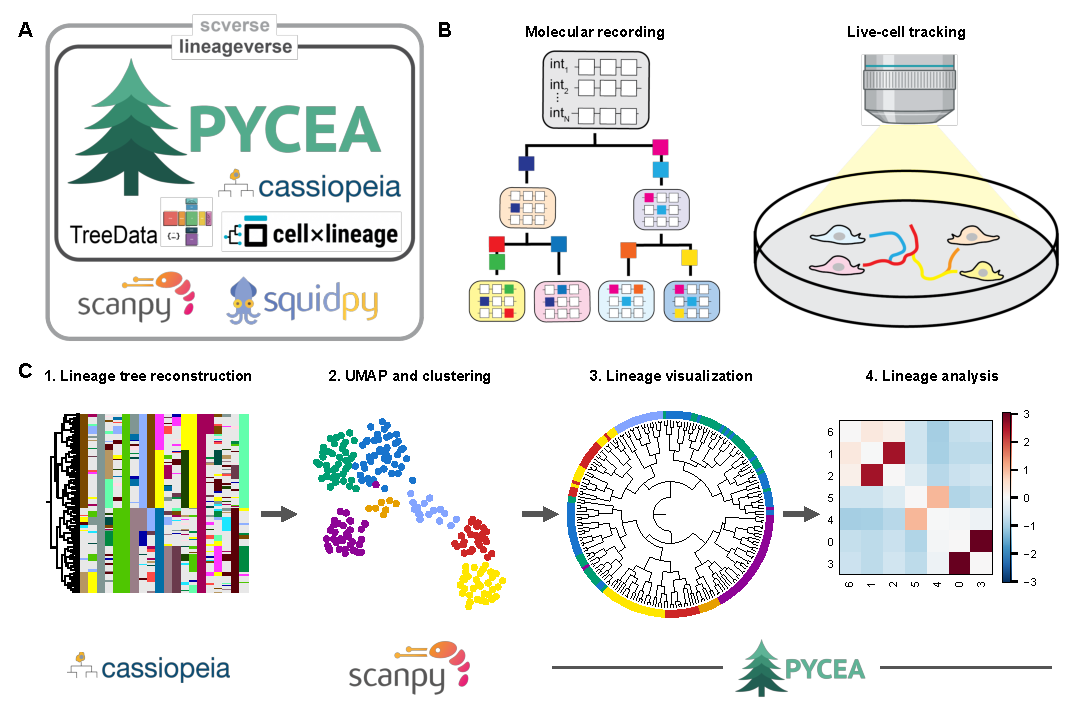
\includegraphics[width=\textwidth]{figure1.pdf}
  \caption{\textbf{Pycea integrates lineage tracing analysis into the scverse ecosystem.}
  \textbf{(A)} Pycea and TreeData within the scverse and lineageverse ecosystems.
  \textbf{(B)} Supported lineage tracing data: molecular recording (left) and live-cell tracking (right).
  \textbf{(C)} Example workflow on single-cell lineage tracing data: (1)~lineage tree reconstruction with Cassiopeia, (2)~UMAP and Leiden clustering with Scanpy, (3)~polar tree with leaves annotated by cluster, and (4)~ancestral linkage between clusters with Pycea.}
  \label{fig:overview}
\end{figure}

\begin{figure}[p]
  \centering
  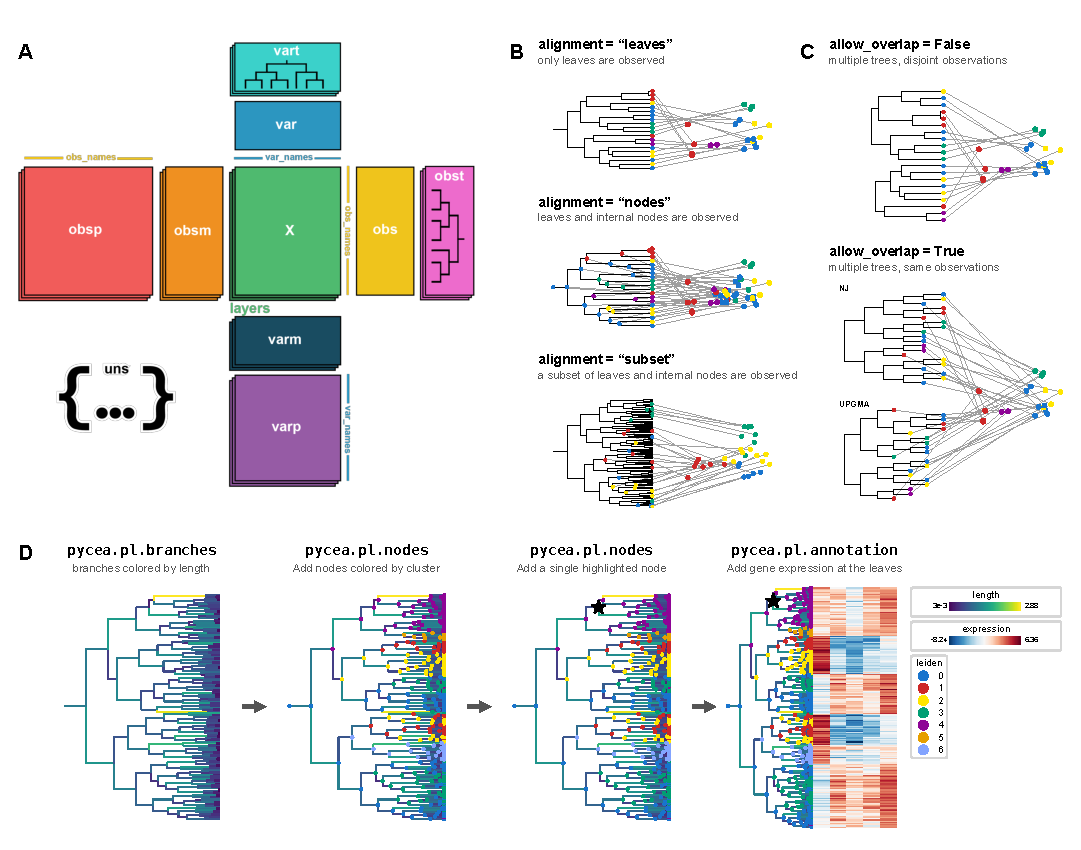
\includegraphics[width=\textwidth]{figure2.pdf}
  \caption{\textbf{The TreeData object stores one or more trees aligned to observations.}
  \textbf{(A)} TreeData extends AnnData with \code{obst} and \code{vart} fields, which store trees aligned to observations and variables.
  \textbf{(B)} Alignment modes. Gray lines connect tree nodes to their observations in the UMAP. With \code{"leaves"}, only leaves are observations; with \code{"nodes"}, leaves and internal nodes are; with \code{"subset"}, only some nodes are.
  \textbf{(C)} Multiple trees per object: trees with disjoint observations (\code{allow_overlap=False}, top) or multiple trees for the same observations (\code{allow_overlap=True}, bottom; neighbor-joining (NJ) and UPGMA).
  \textbf{(D)} A tree plot built up with successive Pycea calls: \code{pycea.pl.branches} (branches colored by length), \code{pycea.pl.nodes} (leaves and internal nodes colored by cluster; then a single node highlighted), and \code{pycea.pl.annotation} (expression of five genes at the leaves).}
  \label{fig:treedata}
\end{figure}

\begin{figure}[p]
  \centering
  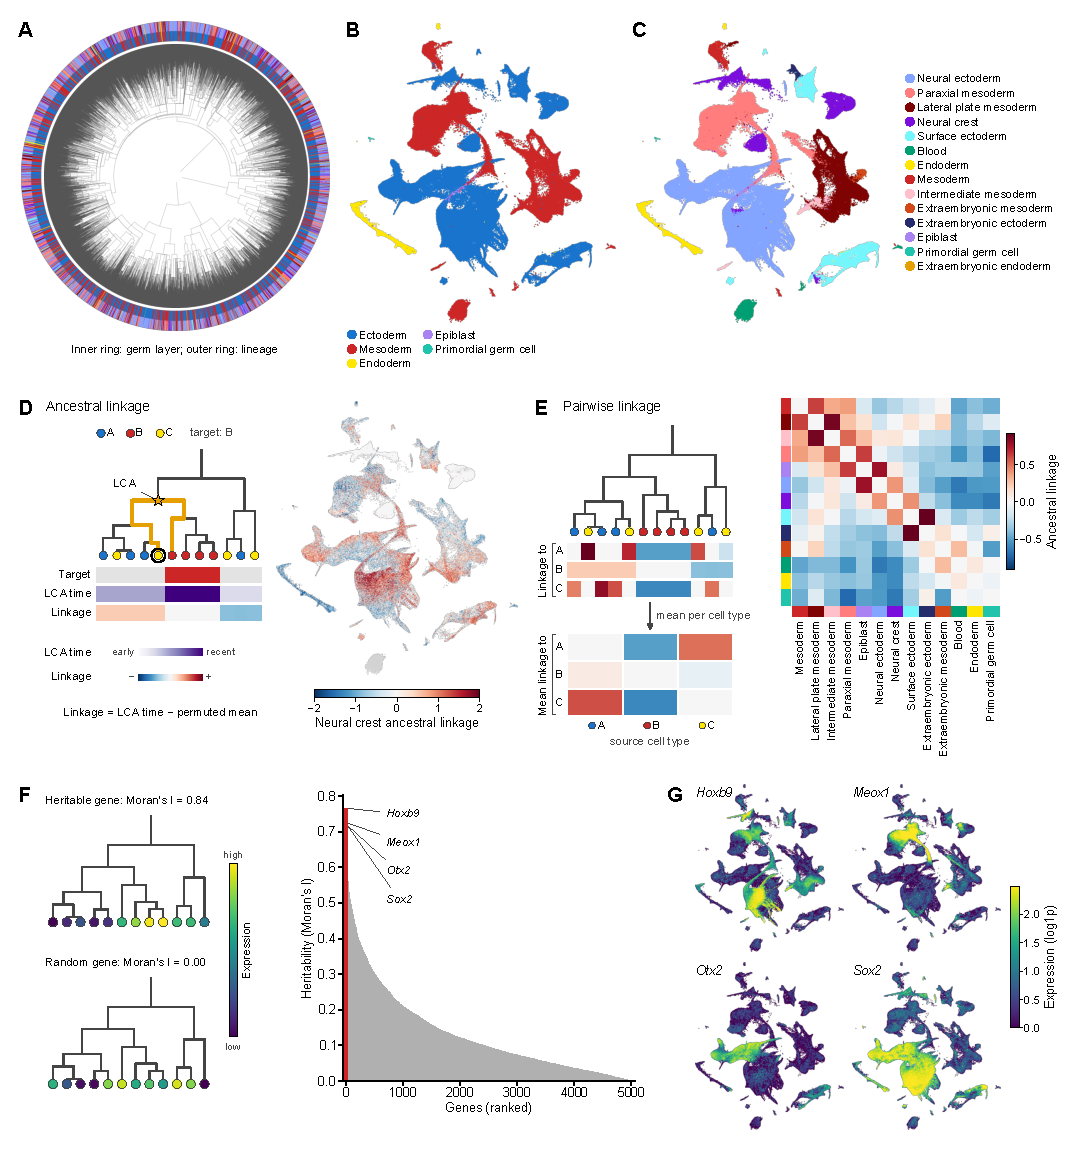
\includegraphics[width=\textwidth]{figure3.pdf}
  \caption{\textbf{Fate restriction in a mouse embryo.}
  \textbf{(A)} Lineage trees of an E9.5 embryo (262,534 cells) with leaves annotated by germ layer (inner ring) and lineage (outer ring).
  \textbf{(B, C)} UMAP of cells colored by germ layer (B) and broad lineage annotation (C).
  \textbf{(D)} Ancestral linkage of a cell to a target set is the time of its most recent common ancestor (LCA) with the nearest target cell, normalized to chance (left). UMAP colored by neural crest ancestral linkage (right); gray cells are not in a lineage tree.
  \textbf{(E)} Pairwise linkage: the mean linkage of each cell type to a target cell type forms one row, repeated with every cell type as the target (left), giving the symmetrized linkage between all lineages (right; colors as in C).
  \textbf{(F)} Heritable genes have expression that is autocorrelated across the lineage tree, measured by Moran's I (left), shown ranked for the 5,000 highly variable genes (right).
  \textbf{(G)} UMAPs colored by expression of the four most heritable genes.}
  \label{fig:embryo}
\end{figure}

\begin{figure}[p]
  \centering
  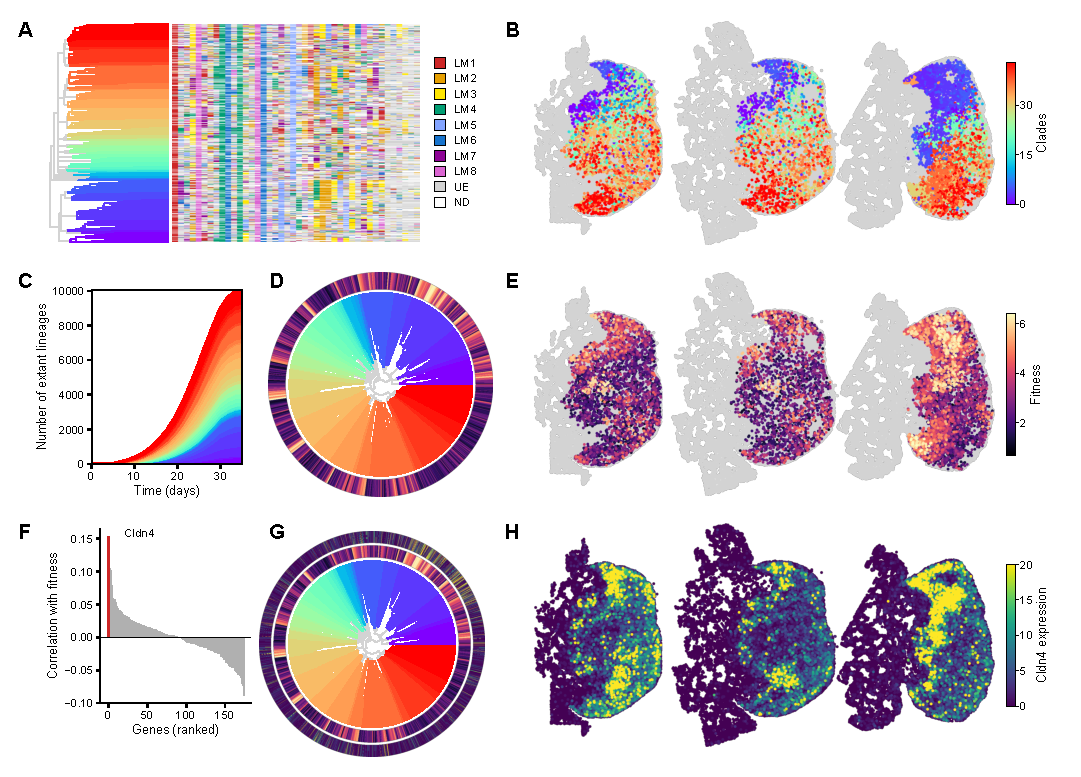
\includegraphics[width=\textwidth]{figure4.pdf}
  \caption{\textbf{Growth dynamics of a 4T1 tumor.}
  \textbf{(A)} Lineage tree and character matrix, with branches colored by clade (cells sharing an ancestor at day 5); colors indicate lineage marks (LMs), gray unedited (UE), and white no detection (ND).
  \textbf{(B)} Spatial distribution of clades across three tumor sections; gray cells are not in the lineage tree.
  \textbf{(C)} Number of extant lineages in each clade over time (\code{pycea.pl.n_extant}).
  \textbf{(D)} Polar tree with the estimated fitness (\code{pycea.tl.fitness}) of each cell in the outer ring.
  \textbf{(E)} Spatial distribution of fitness.
  \textbf{(F)} Correlation of gene expression with fitness; \textit{Cldn4} is highlighted.
  \textbf{(G)} Polar tree with rings for fitness and \textit{Cldn4} expression.
  \textbf{(H)} Spatial distribution of \textit{Cldn4} expression.}
  \label{fig:growth}
\end{figure}

% ---- Supplementary information: figures are numbered S1, S2, ... ----
\setcounter{figure}{0}
\renewcommand{\thefigure}{S\arabic{figure}}
\begin{figure}[p]
  \centering
  {\large\textbf{Supplementary Information}}\par\medskip
  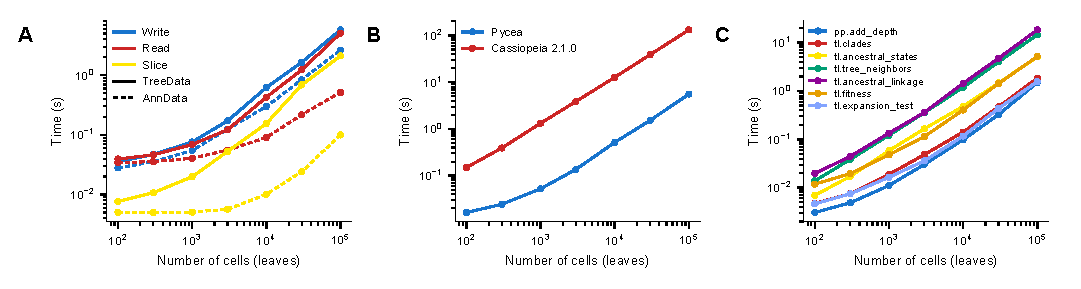
\includegraphics[width=\textwidth]{figureS1.pdf}
  \caption{\textbf{Benchmarks.}
  \textbf{(A)} Time to write, read and slice (a random 10\% of cells) TreeData and AnnData objects with a simulated lineage tree and simulated expression of 20,000 genes (sparse counts), by number of cells.
  \textbf{(B)} Time to plot a tree with Pycea and with Cassiopeia 2.1.0 (plotting deprecated in version 3.0.0), by number of cells.
  \textbf{(C)} Run time of key Pycea functions, by number of cells. Median of three runs, on a single node.}
  \label{fig:benchmarks}
\end{figure}


\end{document}
